\documentclass[14pt, b5paper, twoside]{extbook}
\usepackage[german]{babel}
\usepackage[twoside,bindingoffset=10mm,verbose,marginratio={4:3,5:3},%
textwidth=143.3mm,height=218.6mm, nofoot, showframe]{geometry}


\usepackage{multicol}
\usepackage[hyperfootnotes=false]{hyperref}
\usepackage{pdfpages}
\usepackage{fontspec}
\usepackage{fancyhdr}
\usepackage[compact, bottomtitles]{titlesec}
\usepackage{alphalph}
\usepackage[para, perpage]{footmisc}
\usepackage{footnpag}
\usepackage{graphicx}
\usepackage{svg}
\usepackage{ragged2e}
\usepackage{titletoc}
\usepackage{ifthen}
\usepackage[toc]{multitoc}
\usepackage{etoolbox}
\usepackage{alphalph}
\renewcommand{\thefootnote}{\alphalph{\value{footnote}}}
\renewcommand*{\multicolumntoc}{2}
\patchcmd{\makefootnoteparagraph}
   {\columnwidth}{\textwidth}
   {\typeout{Success}}{\typeout{patch failed}}

\setmainfont[UprightFont       = * ,
             BoldFont          = * Bold ,
             ItalicFont        = * Italic ,
             SmallCapsFont = * ,
             SmallCapsFeatures={Letters=SmallCaps},
             Ligatures=TeX]{Day Roman}

\makeatletter             
\newlength\fake@f
\newlength\fake@c
\def\fakesc#1{%
  \begingroup%
  \xdef\fake@name{\csname\curr@fontshape/\f@size\endcsname}%
  \fontsize{\fontdimen8\fake@name}{\baselineskip}\selectfont%
  \uppercase{#1}%
  \endgroup%
}
\makeatother
\newcommand\fauxsc[1]{\fauxschelper#1 \relax\relax}
\def\fauxschelper#1 #2\relax{%
  \fauxschelphelp#1\relax\relax%
  \if\relax#2\relax\else\ \fauxschelper#2\relax\fi%
}
\def\Hscale{.83}\def\Vscale{.72}\def\Cscale{1.00}
\def\fauxschelphelp#1#2\relax{%
  \ifnum`#1=\lccode`#1\relax\scalebox{\Hscale}[\Vscale]{\char\uccode`#1}\else%
    \scalebox{\Cscale}[1]{#1}\fi%
  \ifx\relax#2\relax\else\fauxschelphelp#2\relax\fi}

\renewcommand{\textsc}[1]{\fauxsc{#1}}

\pagestyle{fancy}
\renewcommand{\sectionmark}[1]{\markright{\thesection~- ~#1}}
\renewcommand{\chaptermark}[1]{\markboth{\chaptername~\thechapter~-~ #1}{}}
\pagestyle{empty}

\fancyhf{}

\fancypagestyle{bible}{%
    \fancyhead{} %Clean headers
    \fancyhead[L]{\leftmark \ \thesection}
    \fancyhead[R]{\thepage}
    \fancyhead[RO]{\leftmark \ \thesection}
    \fancyhead[LO]{\thepage}
}

\fancypagestyle{plain}{%
  \fancyhead{}
  \fancyhead[R, RO]{\thepage}
}

\renewcommand{\chaptermark}[1]{\markboth{\thechapter. {\slshape{##1}}}{}}
\renewcommand{\headrulewidth}{0pt}
% \renewcommand*{\thefootnote}{\alph{footnote}}
\titleformat{\chapter}[hang]{\normalfont\bfseries}{}{0pt}{\Huge}
\titleformat{\section}[wrap]{\bfseries\huge}{}{0ex}{}[]
\titleformat{\subsection}[hang]{\bfseries}{}{0ex}{}[]
\newcommand{\bibleverse}[1]{{\bfseries{#1}}}
\renewcommand{\thesection}{\arabic{section}}
\renewcommand{\chaptermark}[1]{\markboth{\MakeUppercase{#1}}{}}
\setcounter{secnumdepth}{1}
\setcounter{tocdepth}{0}
\global\let\endtitlepage\relax
\makeatletter

\titlecontents{chapter}% <section-type>
[0pt]% <left>
{\bfseries\small}% <above-code>
{\small\thecontentslabel \quad}%<numbered-entry-format>
{}% <numberless-entry-format>
{\small\mdseries\titlerule*[0.75em]{.}\bfseries\contentspage}

\begin{document}

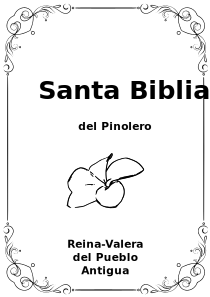
\includepdf{HardCover.pdf}

\null\vfill
\input{../out/tex/00.0-Impressum.tex}
\newpage

\null\vfill
\begin{center}
\begin{minipage}[c]{\textwidth}
  \begin{center}
  \includegraphics{Titel.pdf}
  \end{center}
\end{minipage}
\end{center}
\newpage



\titleformat{\section}[hang]{\bfseries\huge}{}{0ex}{}[]
\input{../out/tex/00.1-Preface.tex}
\titleformat{\section}[wrap]{\bfseries\huge}{}{0ex}{}[]

\tableofcontents
\newpage

\null\vfill
\begin{center}
\begin{minipage}[c]{\textwidth}
  \begin{center}
  \includegraphics{AltesTestamentTitel.pdf}
  \end{center}
\end{minipage}
\end{center}
\null\vfill
\newpage

\pagestyle{bible}

\renewcommand{\cleardoublepage}{}
\renewcommand{\clearpage}{}

\chapter{1. Mose}
\begin{multicols}{2}
  \input{../out/tex/01-1. Mose.tex}
\end{multicols}

\chapter{Psalmen}
\begin{multicols}{2}
  \input{../out/tex/19-Psalm.tex}
\end{multicols}

\chapter{Sprüche}
\begin{multicols}{2}
  \input{../out/tex/20-Sprüche.tex}
\end{multicols}
\newpage

\pagestyle{empty}

\null\vfill
\begin{center}
\begin{minipage}[c]{\textwidth}
  \begin{center}
  \includegraphics{NeuesTestamentTitel.pdf}
  \end{center}
\end{minipage}
\end{center}
\null\vfill
\newpage

\chapter{Offenbarung}
\begin{multicols}{2}
  \parskip=0pt \relax
  \input{../out/tex/66-Offenbarung.tex}
\end{multicols}
\newpage

\end{document}